\subsection{Glyph: \glyph{Perturbation}}
\label{sec:perturbation}

Biochemical networks can be affected by external influences. Those influences can be well-defined physical perturbations, such as a light pulse or a change in temperature; they can also be more complex and not well-defined phenomena, for instance a biological process, an experimental setup, or a mutation. For these situations, SBGN provides the perturbation glyph.

\begin{glyphDescription}

\glyphSboTerm SBO:0000357 ! perturbation

\glyphContainer A \glyph{perturbation} is represented by a modified hexagon
having two opposite concave faces, as illustrated in \fig{af:perturbation}.

\glyphLabel A \glyph{perturbation} is identified by a label placed in an
unbordered box containing a string of characters.  The characters can be
distributed on several lines to improve readability, although this is not
mandatory.  The label box must be attached to the center of the
\glyph{perturbation} container.  The label may spill outside of the container.

\end{glyphDescription}

\begin{figure}[H]
  \centering
  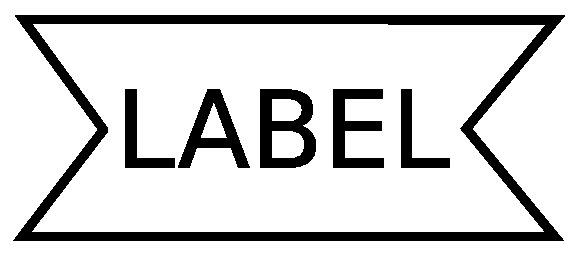
\includegraphics[scale = 0.3]{images/perturbation}
  \caption{The \AF glyph for \glyph{perturbation}.}
  \label{fig:af:perturbation}
\end{figure}
